\documentclass[12pt,letterpaper]{article}
\usepackage{amsmath}
\usepackage{amsfonts}
\usepackage{amsthm}
\usepackage{mathtools}
\usepackage{cancel}
\usepackage[margin=1in]{geometry}
\usepackage{titling}
\usepackage{fp}
\usepackage{enumitem}
\usepackage[super]{nth}
\usepackage{dcolumn}
\usepackage{minted}
\usepackage[title]{appendix}
\usepackage{pgfplots}
\pgfplotsset{compat=1.8}
\usepgfplotslibrary{statistics}

\newcolumntype{d}{D{.}{.}{-1}}

\setlength{\droptitle}{-10ex}

\preauthor{\begin{flushright}\large \lineskip 0.5em}
\postauthor{\par\end{flushright}}
\predate{\begin{flushright}\large}
\postdate{\par\end{flushright}}

\title{STA 032 Homework 1\vspace{-2ex}}
\author{Hardy Jones\\
        999397426\\
        Professor Melcon\vspace{-2ex}}
\date{Winter 2015}

\begin{document}
  \maketitle

  \newmintedfile[rData]{r}{ fontsize=\footnotesize
                          , frame=single
                          }

  \begin{enumerate}[label=(\alph*)]
    \item
      \begin{tabular}{ | l | d | l | r | l | r | }
        \hline
        \multicolumn{2}{| c |}{GPA} & \multicolumn{2}{ c |}{Semester} & \multicolumn{2}{ c |}{Year} \\
        \hline
        Min.    & 1.000 & Fall   & 156             & Min.    & 2007 \\
        1st Qu. & 2.967 & Spring & 352             & 1st Qu. & 2007 \\
        \cline{3-4}
        Median  & 3.250 & \multicolumn{2}{ c |}{} & Median  & 2007 \\
        Mean    & 3.191 & \multicolumn{2}{ c |}{} & Mean    & 2007 \\
        3rd Qu. & 3.500 & \multicolumn{2}{ c |}{} & 3rd Qu. & 2008 \\
        Max.    & 4.000 & \multicolumn{2}{ c |}{} & Max.    & 2008 \\
        \hline
      \end{tabular}

    \item
      \begin{tabular}{ | d | d | }
        \hline
        \text{mean} & \text{standard deviation} \\
        \hline
        3.190807 & 0.4716277 \\
        \hline
      \end{tabular}

    \item
      \begin{tabular}{ | r | r | }
        \hline
        Fall & Spring \\
        \hline
        156 & 352 \\
        \hline
      \end{tabular}

    \item
      There are 508 rows of data.

    \item

      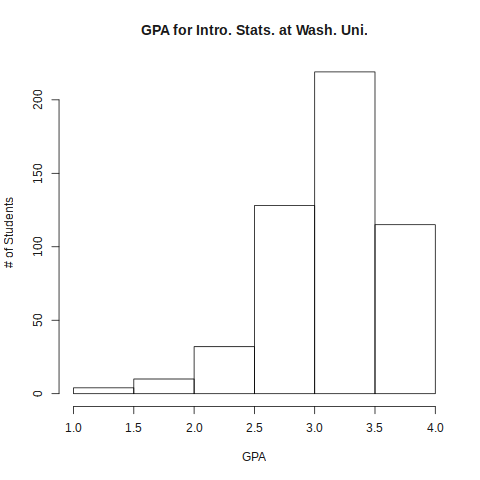
\includegraphics{e.png}

    \item

      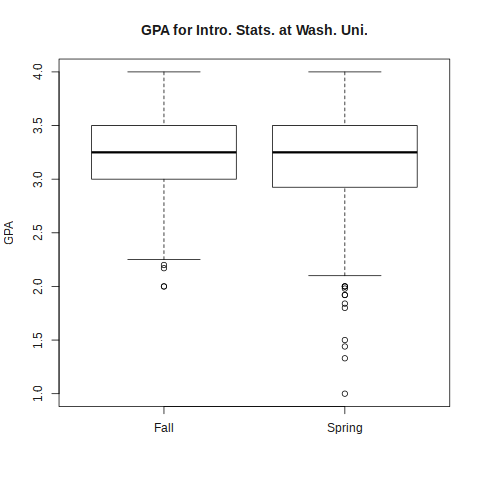
\includegraphics{f.png}

    \item

      \begin{tabular}{| l | l | l | l | l |}
        \hline
            & $Q_1$  & $Q_2$  & $Q_3$  & \nth{90} percentile \\
        \hline
        GPA & 2.9675 & 3.2500 & 3.5000 & 3.7500 \\
        \hline
      \end{tabular}

    \item

      \begin{tabular}{| l | l | l |}
        \hline
            & \nth{5} percentile & \nth{95} percentile \\
        \hline
        GPA & 2.4675             & 3.8725 \\
        \hline
      \end{tabular}

    \item

      \begin{tabular}{| l | l | l |}
        \hline
            & \nth{5} percentile & \nth{95} percentile \\
        \hline
        GPA & 2.25               & 3.84  \\
        \hline
      \end{tabular}

    \item
      Based on the data, it would appear that students have a higher GPA in the fall than they do in the spring.
      This result comes from the fact that the all of the quartiles in fall are higher than they are in the spring,
      and that there are fewer outliers in the fall than there are in the spring.

      However, since this is a sample of 508 students from one college over the course of four semesters,
      this is not indicative one way or the other of the population of students taking introductory statistics.
      More conclusive results could be found by including data from other schools and for more years.
  \end{enumerate}

  \begin{appendices}
    \section{R code}

        \subsection*{Problem 1}
            \rData{prob1.R}
            \subsubsection*{(a)}
                \rData{prob1a.R}
            \subsubsection*{(b)}
                \rData{prob1b.R}

        \subsection*{Problem 2}
            \rData{prob2.R}
            \subsubsection*{(a)}
                \rData{prob2a.R}
            \subsubsection*{(b)}
                \rData{prob2b.R}

        \subsection*{Problem 3}
            \rData{prob3.R}
            \subsubsection*{(a)}
                \rData{prob3a.R}
            \subsubsection*{(b)}
                \rData{prob3b.R}

\end{appendices}

\end{document}
